\documentclass[conference]{IEEEtran}

\usepackage[utf8]{inputenc}
\usepackage{amsmath}
\usepackage{amsfonts}
\usepackage{amssymb}
\usepackage{graphicx}
\usepackage{indentfirst}
\usepackage{algorithm}
\usepackage{algpseudocode}
\usepackage{multirow}
\usepackage{lipsum}
\usepackage{balance}
\usepackage[utf8]{inputenc}
\usepackage{fixltx2e}


\begin{document}

\title{Estimating user activity and sweat rate}
\author
{\IEEEauthorblockN{Lohith Nagaraja}
\IEEEauthorblockA{UID - 304126235 \\
Department of Computer Science\\
University of California, Los Angeles
}
}
\maketitle



\begin{abstract}
Smartphones have been extensively used as a personal activity monitoring device during exercise. This is due to the various sensors that are integrated in the smartphone that provide rich sensor data for native applications to consume in order to infer information about the user, their activity and the surrounding environment. In this paper, we present a model to estimate the sweat rate of an individual according to the intensity level of the exercise activity being performed. The user's performed exercise activity is automatically recognized using accelerometer data from the smartphone in addition to classifying the intensity level. The algorithm is incorporated into our Ultraviolet Guardian (UV-G) system. Our activity classification algorithm on average achieves 90.2\% accuracy. We envision UV-G to serve as assistive healthcare technology, where automated personal recommendations for hydration and sunscreen reapplication will protect the user from sun overexposure and fine grain personal UV exposure history data will be invaluable to skin cancer researchers to correlate long term UV exposure patterns to skin cancer types.
\end{abstract}

\section{Introduction}
Athletes overexerting themselves can overheat by doing too much too fast or trying to endure too long. A 36-year-old female who had been running a marathon was brought to the emergency department (ED) after she had collapsed at the 10 km mark. According to bystander accounts, she was unresponsive, trembling and her eyes were rolling up. On arrival, the patient was noted to be obviously confused and disorientated  \cite{ref1}. In 2011, Josh Lichtle, age 23, died after complications from heat stroke sustained while racing his dirt bike in the 450 class Moto 1 race  \cite{ref2}.

Similar stories also come from the military. In 2003, Private Jason Smith, age 32, a member of the Territorial Army (TA) was found lying face down in an old athletics stadium where he was stationed due to a heat stroke while marching at night and carrying extra weight. He completed just 2.5 miles \cite{ref3}. Running generates about twice the heat of marching. Of 82 heat-stroke cases in Israeli soldiers, 40\% were from brief exercise, as in the first three miles of a run. Over-motivation was a risk factor (Epstein et al., 1999).

Heat illness has received substantial public attention in the United States. Heat stroke is currently the third leading cause of death in athletes behind cardiac disorders and head and neck trauma \cite{ref4}. Early recognition and prompt treatment are keys to the prevention of morbidity and mortality from heat illness. Water is best if the activity lasts less than one hour. For activities lasting more than an hour, a fluid with carbohydrates (sugar) and electrolytes is best. Gatorade and Powerade were designed specifically for rehydration during exercise and contain the right amount of carbohydrates (about 6 \% to 8\%)  \cite{ref5}

 In this paper we look at how we could aid the research aimed towards avoiding dehydration problems, by using smartphones as a feedback device. Smartphones have been used more and more for complex computational tasks in the recent past. Parallelly, the number of smartphone users has been increasing exponentially. According to a recent survey \cite{ref6} the number of smartphone users crossed 835 million in the year 2011. Firms have been constantly striving for innovation in their smartphones, coupled with a whole lot of applications. More and more applications have been created to satisfy ever changing set of user requirements. One such major area of interest happens to be field of personal health and wellbeing. More and more people have been leveraging such applications when exercising, which monitor and store various statistics such as heart rate, calories burnt etc. The users can thus analyze such statistics for a personal review of their exercise cycle. According to a recent survey \cite{ref7} more than 50 percent of smartphone users use their phone while exercising. Thus, there is a constant emphasis in the mobile world to come up with more and more innovative applications to cater to the use of athletes. In this paper we explain an application which would dynamically predict the current activity of the user along with providing vital statistics at the end of the activity cycle. The application makes use of the multi dimensional accelerometer present in the current generation smart phones. The accelerometer can measure acceleration along all 3 dimensions, thereby giving an idea about the device orientation along all 3 coordinates. The accelerometer data vector can be used as a “pattern” to train a classifier, which would then take care of mapping the next set of incoming vectors to the most relevant activity. This classification would aid in the development of custom applications such as report generator, calorie intake advisor etc.

One such application is the prediction of water loss in the form of sweat rate - based upon the user activity.The human body has a self-regulating mechanism in order to maintain adequate body temperature based on the environmental factors \cite{ref8} . This is accomplished by various mechanisms such as convection, conduction, radiation and evaporation. The extent to which a particular mechanism contributes to heat regulation depends on the scenario. However while exercising; evaporation is the predominant heat regulation mechanism. Studies indicate evaporation contributes as much as 80 percent when it comes to removing the excess heat from the body during exercise \cite{ref8}. Evaporation is a heat dissipating mechanism, where in water is lost from the body in the form of sweat. Heat is lost in this process as the water is converted from liquid state to gaseous state and it escapes through the skin. For every 100ml of water lost in the form of sweat, the body temperature is reduced by 1 degree C, thus compensating the external environment temperature variations. It has been estimated that sweat rate can exceed 2 liters per hour during competitive sport. It can reach peaks of 3-4 per hour liters for a very short duration during high intensity exercise. Adequate amount of fluid intake is to be provided to the human body to compensate this water loss, to avoid problems related to dehydration and water loss. Human body is made of 75\% water, some of which is lost at regular intervals from the body in the form of respiration, sweat and waste elimiation \cite{dehydration1}. Dehydration sets in when there is a failure to adequately replace this loss in the form of fluid intake. It also indicates the status of a human body, where in the water loss is to such an extent as to cause decrease in the blood volume levels. This would decrease the efficiency of the human circulatory system to provide oxygen to various parts of the body. Studies indicate capacity to perform high-intensity exercise reduces by as much as 45\% when dehydration loss is only 2.5\% of body weight \cite{dehydration2}. Table 1 explains in detail the various ill effects dehydration would cause \cite{ref9}.


\begin{table}[htbp]
\centering
\begin{tabular}{|c|l|c|c|c|}
\hline 
\textbf{\rule{0pt}{4ex} Body weight loss \%} & \textbf{\rule{0pt}{4ex}Ill effects}\\
\hline
\rule{0pt}{4ex}1-2 & Thirst, Fatigue and weak physical performance  \\
\hline
\rule{0pt}{4ex}3-4 & Nausea and decrease in blood volume  \\
\hline
\rule{0pt}{4ex}5-6 & Heading and breathing difficulties  \\
\hline
\rule{0pt}{4ex}7-8 & Dizziness and error in mental judgement  \\
\hline
\rule{0pt}{4ex}9-10 & Exhaustion and death  \\
\hline
\end{tabular}
\bigskip
\caption{Water loss in terms of body weight and subsequent ill effects}
\par
\bigskip
\end{table}

Estimating sweat losses would also help in several establishments such as calculating water needs in military establishments \cite{ref10} . Part of military planning would involve providing adequate amount of water to the personnel. Too little water, the soldiers can be dehydrated. If too much water is provided, it could curtail their fighting capabilities since it could add extra baggage weight which could be a hindrance in difficult terrains. In fact military establishments use existing equations to estimate the sweat rate based on existing conditions and provide the required amount of water. In this paper we would explain why existing equations would be difficult to transform into an android application and we also explain a new approach to notify the users when their sweat rate tends to get higher.

In the next section we would provide an overview of some of the key elements and constructs used in the application development process. Later we explain the methodologies behind the application which would predict the exercise the user is performing. Our focus later shifts to sweat rate estimation, where in we explain the existing methods and limitations when it comes to incorporating them into android. We later present a simple approach to compute the sweat rate based on the user activity which is obtained via our prediction model.

\section{Overview}

\subsection{Android Sensors}

Android provides several sets of motion sensors which are either hardware or software based \cite{ref11} . These sensors monitor the motion of the device and measure the relevant data parameters. The hardware based sensor includes the accelerometer and the gyroscope. Other sensors such as the gravity, linear acceleration, and rotation vector sensors can either be hardware based or software based. Motion sensor determines the device movement pattern such as rotation and shake. Motions can either be due to users input (such as shaking the device) or due to physical environment change (such as user running with the device). Motion sensors when enabled and utilized, return an array of sensor values.

Android provides several sets of environment sensors as well which give information about the local environment. These sensors are hardware based – dedicated to a specific parameter. The current android platform supports sensors for relative ambient humidity, luminance, ambient pressure, and ambient temperature. Unlike motion sensors, for each sensor event the environment sensors return a single specific value rather than an array of values.


\subsection{Weka classifier}
Waikato Environment for Knowledge Analysis (WEKA) is open source software written in java, which supports data mining \cite{ref12}. WEKA contains a set of visualization tools and machine algorithms written around data analysis and predictive modeling. The WEKA also provides several UI features, which ease the analysis and usage process. Weka supports several data mining concepts such as data preprocessing, clustering, regression, visualization, classification and feature selection.
\section{Predicting User activity}

\subsection{Using the accelerometer}

In order to predict the user activity, accelerometer data would be used for the required calculations. Current generation smartphones are equipped with accelerometers, which were intially used for applications such as gaming to track motion. However as applications evolved, they made use of accelerometer data for specialzed tasks such as tracking and generating feedback. Accelerometers are capable of tracking the phone movements continously along all 3 Dimensions. In our application, we use this data to calculate the magnitude of the user movement. As explained earlier android provides the required hardware based sensors to obtain this value. 

\begin{figure}[H]
\centering
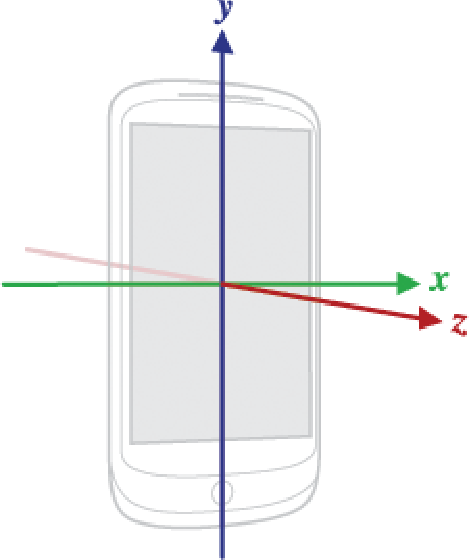
\includegraphics{axis_device.pdf}
\caption{Accelerometer measures movements along all 3 dimensions}
\end{figure}

As showin in figure 1, Accelerometers estimate the acceleration force along all the 3 dimensions. Our application subscribes to the sensor changes through a event handler. Each time a linear acceleration sensor event is raised, the event handler records the sensor sample(x,y,z). Accelerometer magnitude can be obtained from this sample as follows:

\begin{equation}
m = \sqrt{x^2+y^2+z^2}
\end{equation} 

where x is the acceleration force along the x axis, y is the acceleration along y axis and z is the acceleration force along the z axis.


\begin{figure*}
\centering
  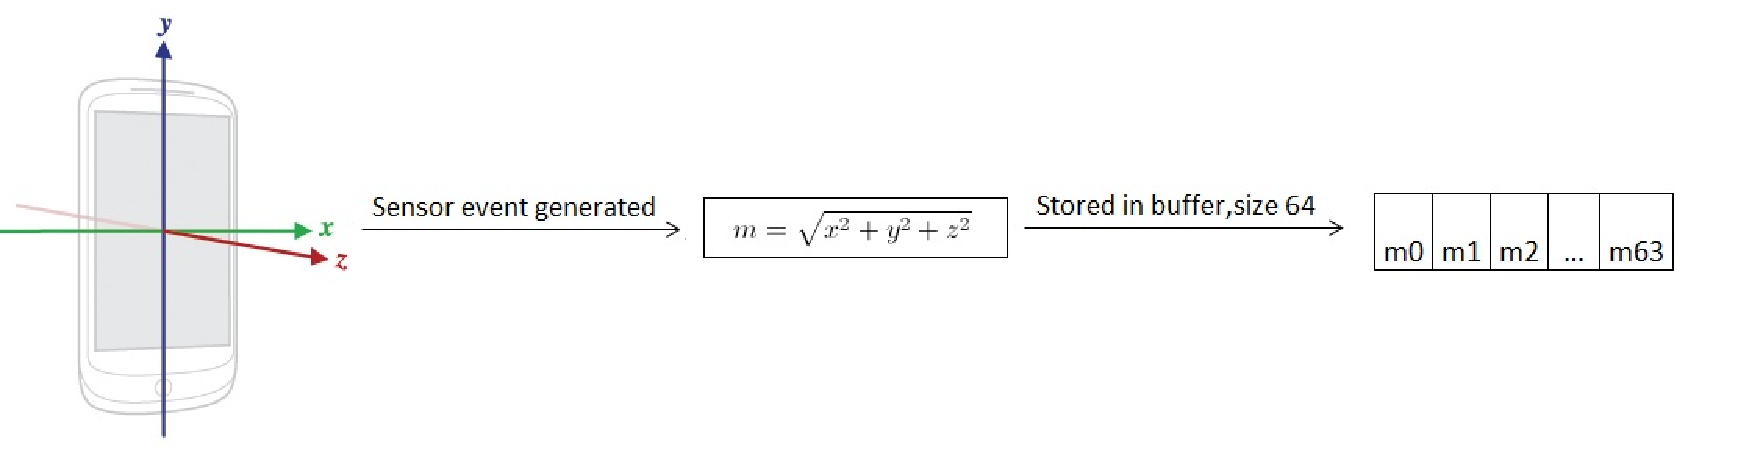
\includegraphics[width=6in,height=1.6in]{sensor_to_buffer.pdf}
  \caption{Accelerometer magnitude calculation.}
\end{figure*}


As shown in Figure 2, Once the magnitude is calculated the value is stored in a work flow buffer of pre-defined size, which has been set to 64 in the application. Once the buffer is full, the next step would involve calculating fourier transforms required for the classifier algorithm.

\subsection{Generating fast fourier transform}

\begin{figure*}
\centering
  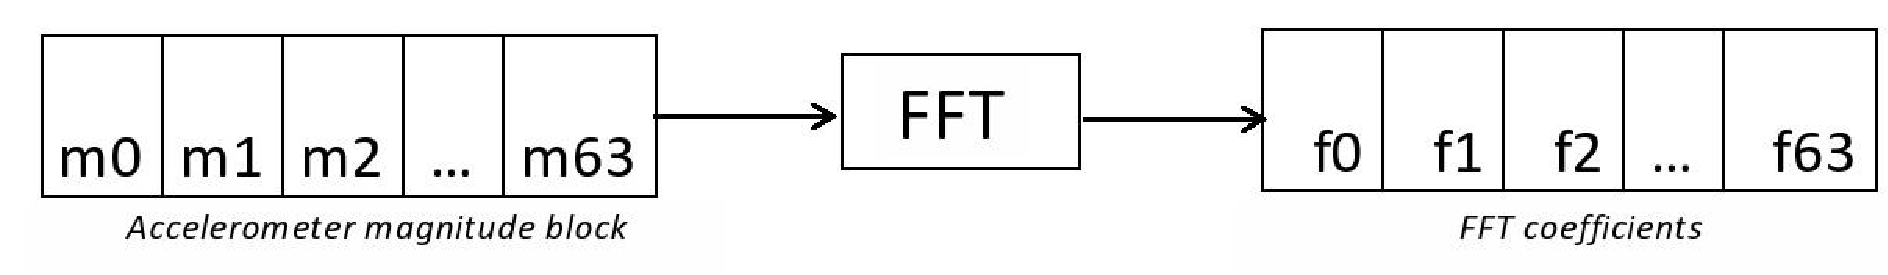
\includegraphics[width=5in,height=0.6in]{magnitude_to_fft.pdf}
  \caption{FFT coeffcient calculation for the training phase.}
\end{figure*}

We compute fast fourier transform (FFT) feature for each of the magnitude readings(m0...m63) as shown in figure 3, which would then be used in the training and classification phase as we would see in the next section.Each of the computed feature is referred to as the FFT coefficients(f0...f63). FFT is responsible for transforming a time series of amplitude over time to magnitude, across frequency.

\subsection{Training and classifying using weka}

In this section we provide an overview of how Weka is used in collaboration with the FFT coefficients in both the training phase and the classifier phase.

\begin{figure*}
\centering
  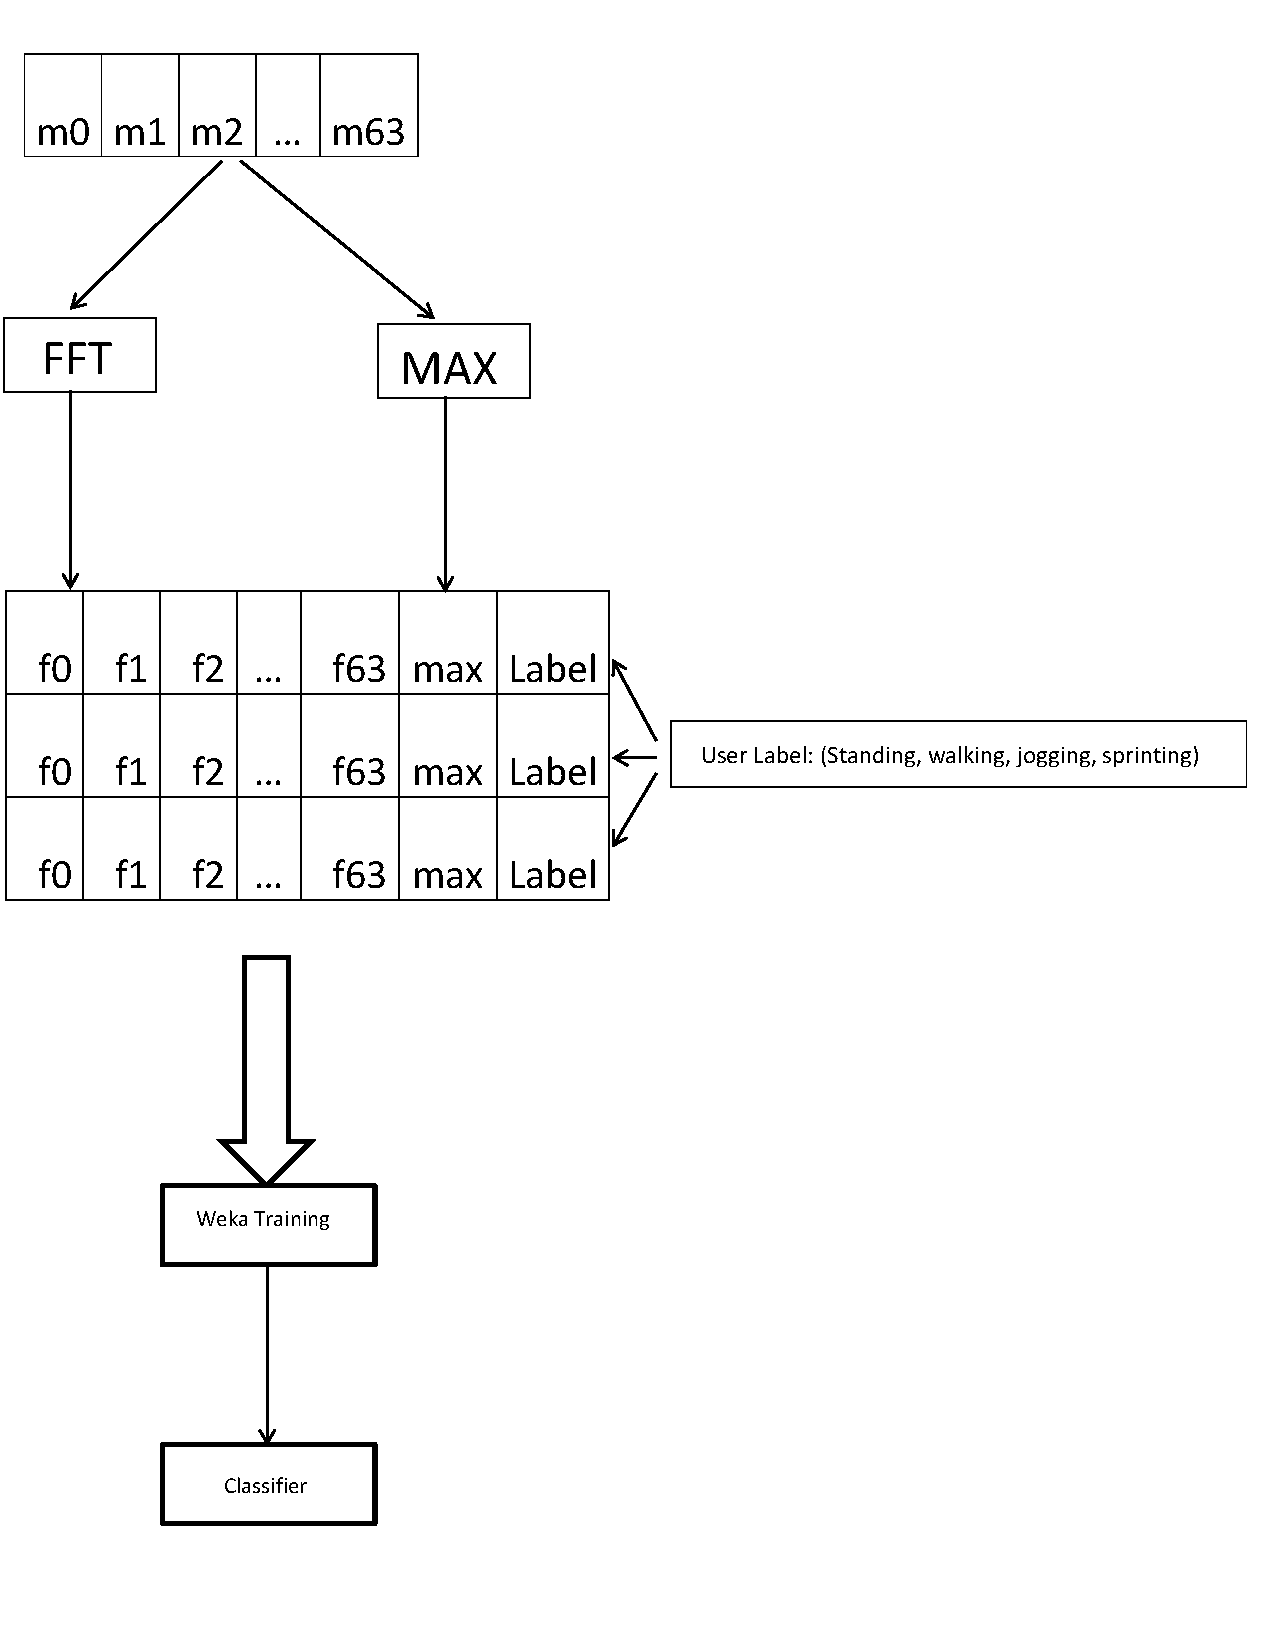
\includegraphics[width=5in,height= 7in]{magnitude_to_feature_vector.pdf}
  \caption{Training and classifier creation. }
\end{figure*}

For the training phase, we use an utility android application. A simple representation of the work flow can be seen as represented in figure 4. The user can collect the data using the test application by specifying a label which indicates the activity the user is performing. As and when the user is performing the exercises, The training module calculates the FFT coefficients and also stores calculates the maximum among the corresponding magnitude values in the buffer(MAX). The FFT coefficients (f0.. f63), MAX and the specified label together constitute a feature vector. The number of feature vectors would be directly proportional to the time the user spends in performing the activity . Once the user opts to end data collection, training module would format all the feature vectors into arff file format as required by the Weka classifier.

In order to complete the training phase, the training data set is uploaded on Weka GUI and the appropriate algorithms choosen. Based on the algorithm chosen, the corresponding classifier is generated. In case the we choose J48 algorithm - we can also generate the classifier source code in java. This classifier is incorporated into our android application and used in the classifier stage.

\begin{figure*}
\centering
  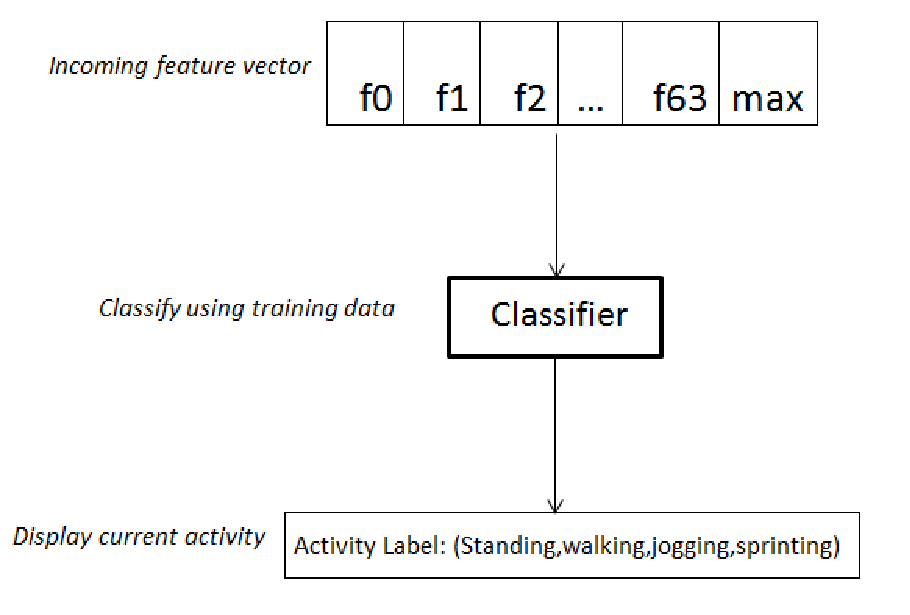
\includegraphics[width=3in,height= 2in]{feature_vector_to_activity.pdf}
  \caption{Using the classifier to determine a user activity.}
\end{figure*}
The workflow during the classification module is as shown in figure 5. In this scenario, the application again computes the feature vectors as and when the user is performing the exercises. However the feature vectors do not specify any user label. Once the feature vectors are collected, the application makes use of the trained classifier to analyze the feature vector and hence compute the corresponding label. This label is displayed to the user to indicate the current activity being performed. Also the application factors in all the feature vectors till the user opts to stop the application and computes a dominant activity using the classifier. This would indicate the activity the user spent the maximum time on in the current exercise cycle.

All the stages involved in identifying user activity are summarized step by step in figure 6.

\begin{figure*}
\centering
  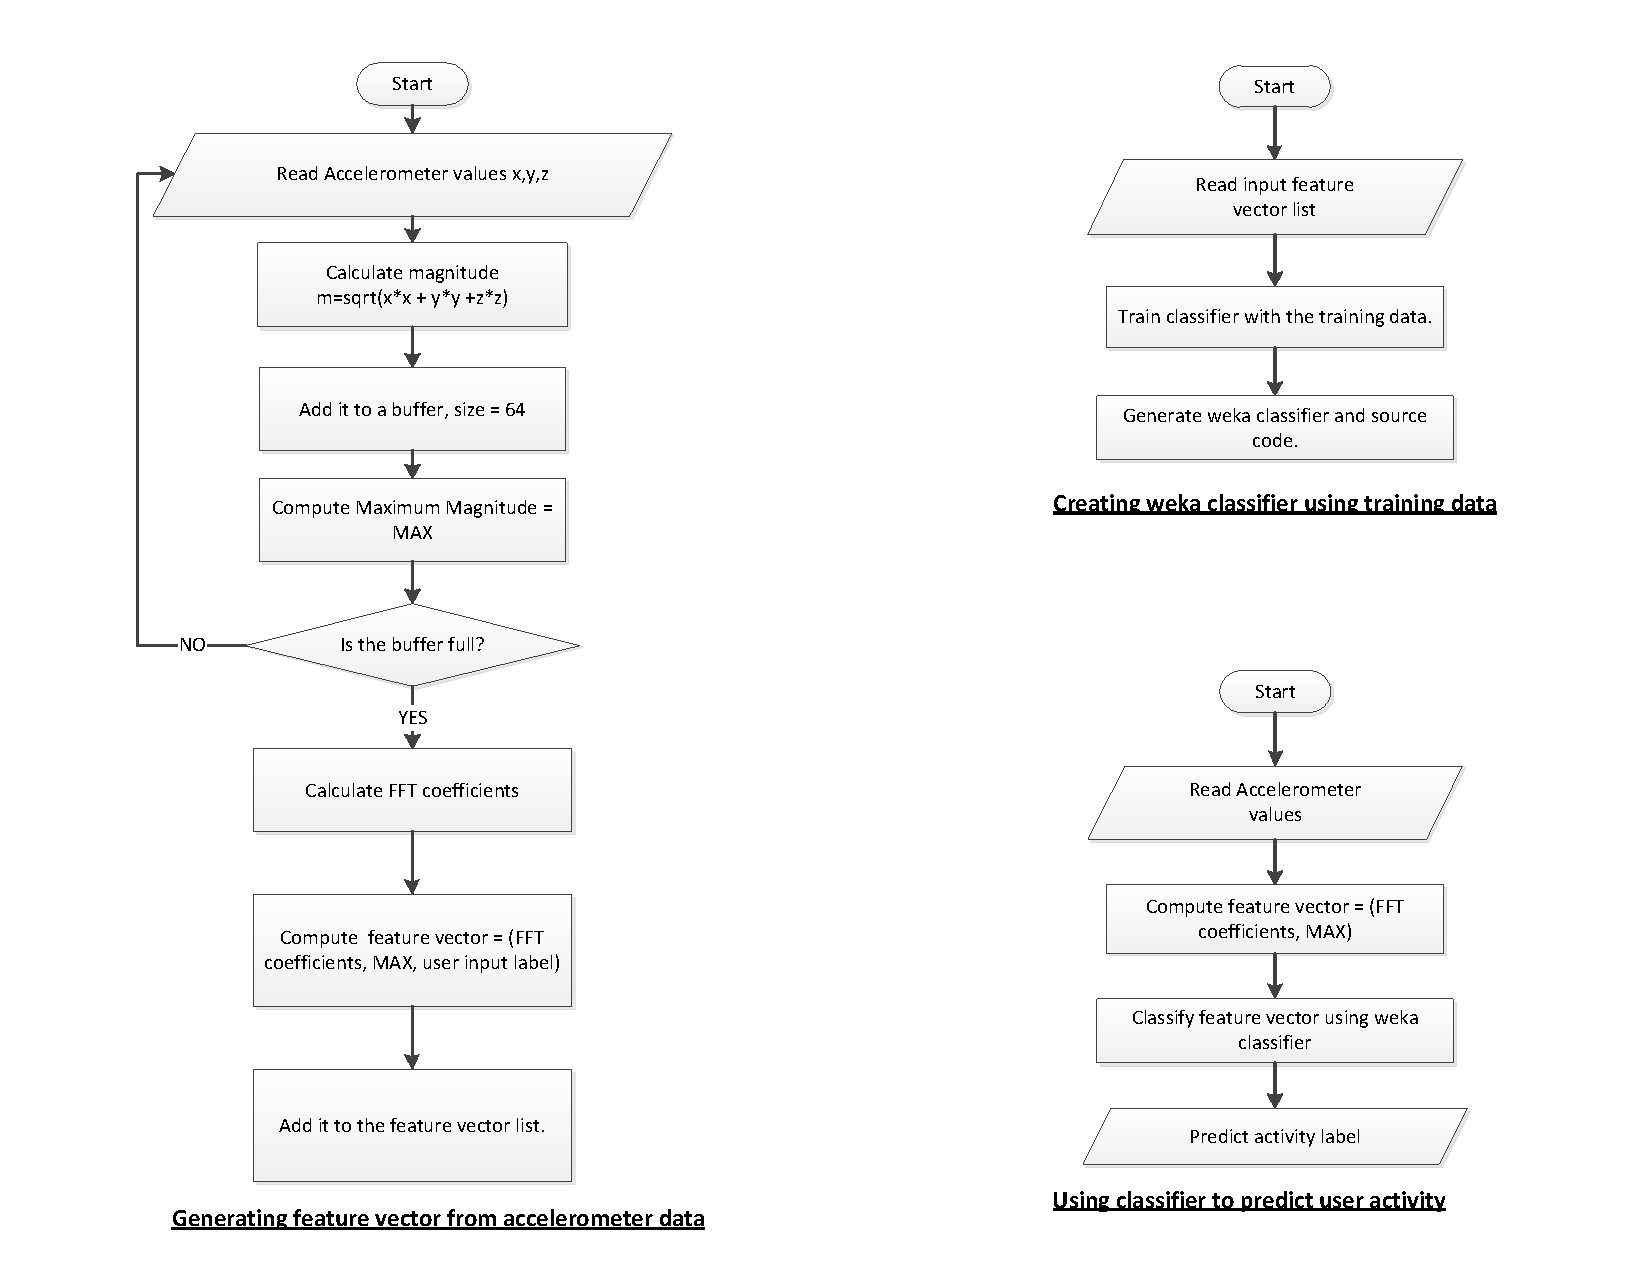
\includegraphics[width=\textwidth,height=5in]{algorithm1.pdf}
  \caption{Overview of the activity identification process. }
\end{figure*}

\subsection{Application overview}
The android application environment included a Samsung galaxy S4 smartphone, equipped with Jelly bean version of android. The application utilizes the various sensors of the smartphone. Primary among them is the Motion sensor which would be used to calculate the linear acceleration. To facilitate the same, the application internally registers event handling modules with the corresponding sensors of the devices. In order to train the weka, data was collected by performing various activities in UCLA. Each activity (Standing, walking, jogging, sprinting) was performed for a duration of at least 30 seconds and repeated several number times  under different stress conditions to ensure a good amount of data to train the classifier. The phone was wrapped near the bicep region of the subject, again to avoid interference. As indicated earlier an utility android application was used to collect the training data by pre specifying the activity. A snapshot of the application can be seen figure 7. The screenshot shows the current activity being performed by the user as well as the corresponding estimated sweat rate. In the next section we are going to explain how we arrived at this sweat rate projection. The user can either opt to save the exercise profile, or cancel the data collection. The application would save the relevant details such as dominant activity, which the user can choose to examine later.



\begin{figure*}
\centering
  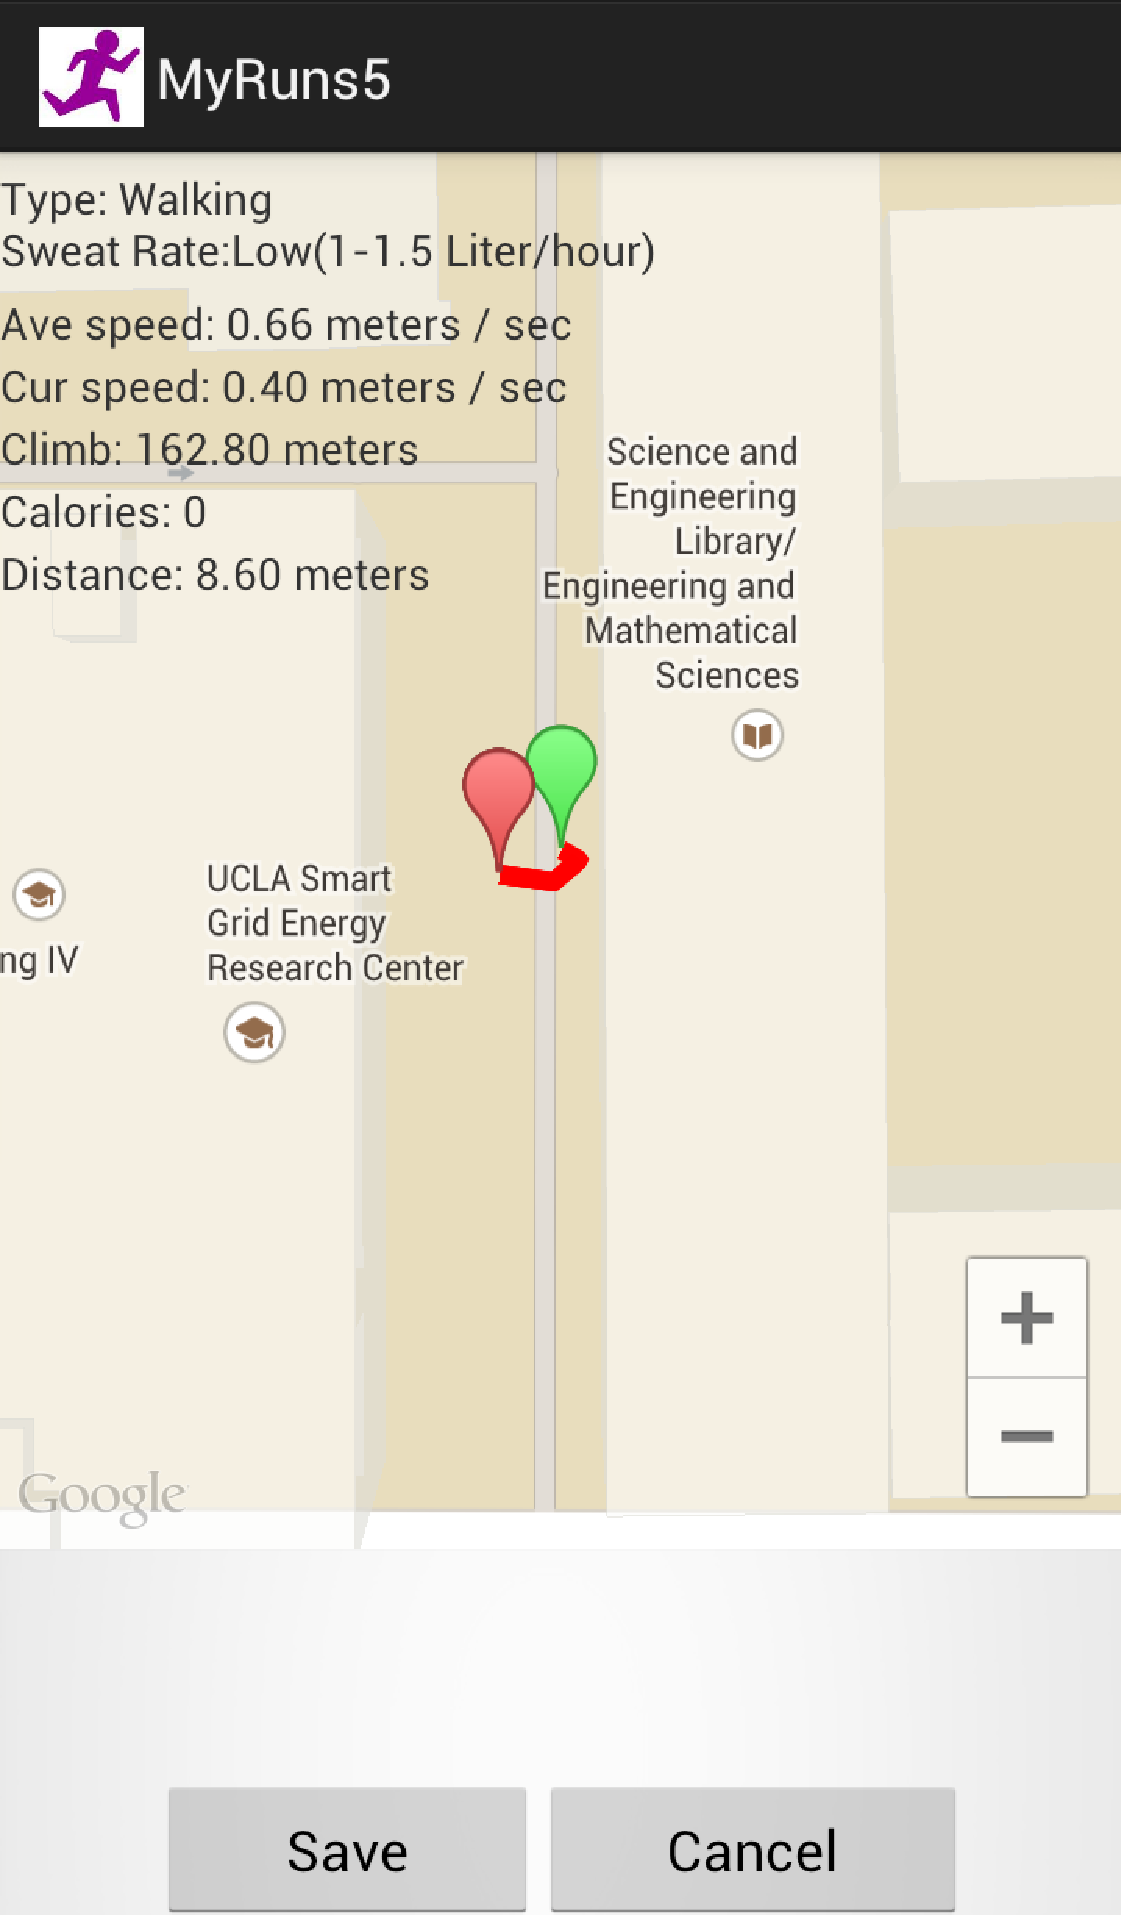
\includegraphics[width=2in,height=3in]{app_screen_shot.pdf}
  \caption{A snapshot of the application.}
\end{figure*}

\section{Predicting sweat rates}
\subsection{sweating in humans}
During a state of rest or an exercise, human body can lose water either through Trans epidermal loss or sweating. The Trans epidermal loss is unrelated to the water lost due to sweat and on an average – the whole body transepidermal water loss is around 30 grams per hour \cite{sweat1}. The loss of water through skin (due to evaporation and other factors) contributes to around 50 percent of this loss. The majority of this loss can be attributed to hands and feet portion of the human body. In fact – studies indicate the loss through these body parts can be two four times as high, when compared to loss through the other body parts.
Water loss due to sweat is due to the sweat glands spread all over the body. The distribution of sweat glands is non-uniform and thus characterizes the non – uniform distribution of sweat all over the body. For example, Hands and feet count for only 5.2 percent of total body surface area, yet they possess 25 percent of total sweat glands.
The total amount of sweat loss would vary depending on the sort of exercise the body is being subjected to. In men, it can exceed 2 Liters per hour during competitive sport. Also the sweat rate can hit highs of 3-4 liters per hour for a very short duration during such high intensity exercise. Studies also indicate, Sweat secretion is generally more in the evening then in the morning. Over the course of several experiments in the past – several approaches have been used to measure sweat rate – such as filter papers and specialized capsules. A collaborative analysis of all the approaches indicates – the mean sweat rate in case of a resting body is determined on an average to be around .36 mg/cm-square/minute. The same rises to around .89 mg/cm-square/minute when the body is subjected to physical exercises.

\subsection{Existing methods to predict sweat rate}

Several approaches have been used to calculate sweat rate in humans while exercising. The most common and easiest approach is to measuring the weight differential using the following equation:

\begin{equation}
mean\_sweat\_rate=\dfrac{(W_{dif}+F_{in})}{E_{dur}}
\end{equation}

where, W\textsubscript{dif} indicates the difference in weight before and after exercise, F\textsubscript{in} indicates the fluid intake during the exercise cycle and E\textsubscript{dur} indicates the duration of the exercise cycle.

 However in order to provide a feedback to a user during exercise, we would need a mechanism to calculate the sweat rate dynamically as and when the user is exercising. There are several other approaches which use specialized sensors to monitor sweat rate. These sensors generally estimate the local environmental factors such as local temperature and air pressure to estimate the sweat rate \cite{sweat2}.Equations have been formulated taking into consideration several factors which influence sweat rate. These factors include environmental traits such as temperature, air pressure and user traits such as clothing, velocity, Climb grade, mass etc. The equations thus formulated take into consideration maximum evaporative capacity of the environment as well as evaporation required to maintain heat balance. The following is an equation(known as Shapiro sweat prediction equation) to calculate the mean sweat rate \cite{sweat3}:

\begin{equation}
mean\_sweat\_rate = 27.9 \times E_{req} \times (E_{max})^{-0.455}
\end{equation}

where E\textsubscript{req} indicates the Evaporation required to maintain heat balance and E\textsubscript{max} indicates maximal evaporative capacity of the environment.

The above equation has been validated in several different environmental setups. One such experiment conducted extensive tests \cite{sweat4} and corrected the equation as follows:

\begin{equation}
mean\_sweat\_rate = 147+1.527 \times E_{req}-0.87 \times E_{max}
\end{equation}


Both sets of equations have been extensively tested and give a good approximation of the sweat rate. However in order to compute these values, we need several parameters including user traits such as weight and clothing information as well environmental traits such as temperature, air velocity and pressure. 

Both sets of equations have been extensively tested and give a good approximation of the sweat rate. Ideally we would want to incorporate them into our android application. However we came across several constraints which hampered the same.

One of the main parameters needed to calculate sweat rate using (3) and (4) was the local environment characteristics where in the user is performing such exercises. Though weather APIs can be used to get parameters such as humidity and air velocity in a particular location, it may be difficult to achieve granularity to the particular location and local environment where the user is exercising. Another important parameter for the environmental heat load calculation was the estimation of thermal resistance of clothing, which cannot be measured with the current sensor framework of android. Metabolic rate calculation is another important aspect in calculating sweat rate and it requires several traits of the user such as user speed, current weight as well as grade differential. Though there are ways to calculate user speed through accelerometer sensors and GPS , they are plagued by problems of inaccuracy. The degree of inaccuracy increases as the user covers more distance and makes twists and turns. The user is also constrained to enter the weight before starting the exercise. Also since the user may lose significant weight once the exercise is started, the degree of error could increase. Calculating grade differential would involve altitude change and distance covered by the user – which once again has a high level of inaccuracy in the present android framework.
 
Due to all these limitations, the existing equations cannot be incorporated into an android application to calculate the user sweat rate. In this project we have estimated the sweat loss based on the activity obtained from the classifier. Using this simple model, we avoid the complexities involved in calculating the sweat rate using the classic equations such as (3) and (4).

\subsection{Predicting sweat rate based on activity analysis}
Since there are quite a few number of constraints involved in incorporating the existing sweat rate prediction equations into Android, we came up with a simple approach to predict the level of sweating. We collaborated various research papers, their studies and experiments \cite{sweat5}  \cite{sweat6} and approximated the average sweat rate based on the activity to be performed. Table 2 summarizes the details of the sweat rate averages for these activities



\begin{table}[htbp]
\centering
\begin{tabular}{|c|l|c|c|c|}
\hline 
\textbf{\rule{0pt}{4ex} Activity type} & \textbf{\rule{0pt}{4ex} Average sweat rate(Liters per hour)} \\
\hline
\rule{0pt}{4ex}  {Standing} & 1.5 \\
\hline
\rule{0pt}{4ex}  {Walking} & 1.5 \\
\hline
\rule{0pt}{4ex}  {Jogging} & 2.0  \\
\hline
\rule{0pt}{4ex}  {Spriting} & 3.0  \\
\hline
\end{tabular}
\bigskip
\caption{Average sweat rate obtained for different activities}
\par
\bigskip
\end{table}


Based on these observations, we incorporated this approximation model in our application. Since we already have in place mechanism to classify the current activity being performed, as well the dominant activity in the current exercise cycle - we would perform a simple mapping. We would identify the duration for which the dominant activity has been performed, and calculate the total amount of sweat lost accordingly. In the current implementation, we would obtain the dominant activity every minute. Based on  the  this dominant activity and its total duration we would correspondingly calculate the total amount of sweat lost based on table 2.

Mathematically this approximation can be represented using the following equation:

\begin{equation}
total\_sweat\_rate=\sum{\dfrac{(msr_{a} \times t_{a})}{3600}}
\end{equation}

where  total\_sweat\_rate   indicates the total amount of sweat lost by the user over the course of the exercise.  msr\textsubscript{a} indicates the mean sweat rate of the dominant activity in that minute, based on table 2. t\textsubscript{a} indicates the time in seconds the dominant activity has been performed.

\section{Results and Analysis}

In this section we are going to provide a brief overview of the prediction model. We analyze the accuracy of the activity predictor, by using various algorithms. We also analyze the limitations involved in establishing the accuracy of sweat rate estimation.

\subsection{Activity prediction analysis}

Weka classifier has a self evaluation module, to calculate the accuracy of the prediction model it constructs. Once the classifier is constructed, weka would once again back track to classify the instances in the training data to predict the activity. Since the training data set already has the actual activity - the classifier can thus evaluate the accuracy of the prediction algorithm used. In the following section, we compare the accuracies of several algorithms which can be used as a predictor in our application. 


Table 3 provides the number of  samples we took for each activity.

\begin{table}[htbp]
\centering
\begin{tabular}{|c|l|c|c|c|}
\hline 
\textbf{\rule{0pt}{4ex} Activity type} & \textbf{\rule{0pt}{4ex} Number of samples)} \\
\hline
\rule{0pt}{4ex}  {Standing} & 206 \\
\hline
\rule{0pt}{4ex}  {Walking} & 209 \\
\hline
\rule{0pt}{4ex}  {Jogging} & 332  \\
\hline
\rule{0pt}{4ex}  {Spriting} & 363  \\
\hline
\end{tabular}
\bigskip
\caption{Number of activity collected for different activities}
\par
\bigskip
\end{table}



Table 4 map the accuracy provided by some of the weka algorithms against the set of activities to identified.\\


\begin{table}[htbp]
\centering
\begin{tabular}{|c|l|c|c|c|}
\hline 
\textbf{\rule{0pt}{4ex} Algorithm} & \textbf{\rule{0pt}{4ex} J48} & \textbf{Multilayer perception} & \textbf{Decorate}& \textbf{ASC} \\
\hline
\rule{0pt}{4ex}  \textbf{Average} & 90.2 & 87.6 & \textbf{91.1} & 91  \\
\hline
\end{tabular}
\bigskip
\caption{Comparision of accuracies obtained by different classifier algorithms}
\par
\bigskip
\end{table}

As evident from the table, we get a fairly good deal of accuracy when it comes to activity prediction.Detailed analysis indicates standing and walking enjoy higher degree of accuracy compared to the other set of activities.However jogging and sprinting enjoy accuracy to a lesser degree.  An obvious thought of reasoning could be that , since Jogging is similar to sprinting, especially when the sprinter slows down - this could give rise to inconsistencies.  An analysis of the confusion matrix for the various algorithms confirms this line of reasoning as we would see next. Confusion matrix is one more algorithm prediction analysis feature provided by Weka. In this matrix, the sets of classes are mapped against each other to indicate the number of instances one of them were confused with the other by the algorithm. For ex : In table 5, for J48 algorithm walking activity was confused with sprinting on 7 occasions.\\


\begin{table}[htbp]
\centering
\begin{tabular}{|c|l|c|c|c|}
\hline 
 & \textbf{\rule{0pt}{4ex} Stand} & \textbf{Walk} & \textbf{Jog}& \textbf{Sprint} \\
\hline
\rule{0pt}{4ex} Stand & 193 & 1 & 0 & 12 \\
\hline
\rule{0pt}{4ex} Walk & 1 & 200 & 1 & 7  \\
\hline
\rule{0pt}{4ex} Jog & 0 & 4 & 298 & \textbf{30} \\
\hline
\rule{0pt}{4ex} Sprint & 14 & 8 & \textbf{31} & 310  \\
\hline
\end{tabular}
\bigskip
\caption{Confusion matrix for J48 algorithm}
\par
\bigskip
\end{table}


\begin{table}[htbp]
\centering
\begin{tabular}{|c|l|c|c|c|}
\hline 
 & \textbf{\rule{0pt}{4ex} Stand} & \textbf{Walk} & \textbf{Jog}& \textbf{Sprint} \\
\hline
\rule{0pt}{4ex} Stand & 185 & 0 & 0 & 21 \\
\hline
\rule{0pt}{4ex} Walk & 2 & 198 & 0 & 9  \\
\hline
\rule{0pt}{4ex} Jog & 3 & 1 & 295 & \textbf{33} \\
\hline
\rule{0pt}{4ex} Sprint & 40 & 3 & 26 & 294  \\
\hline
\end{tabular}
\bigskip
\caption{Confusion matrix for Multi layer perceptron}
\par
\bigskip
\end{table}

\begin{table}[htbp]
\centering
\begin{tabular}{|c|l|c|c|c|}
\hline 
 & \textbf{\rule{0pt}{4ex} Stand} & \textbf{Walk} & \textbf{Jog}& \textbf{Sprint} \\
\hline
\rule{0pt}{4ex} Stand & 197 & 0 & 0 & 9 \\
\hline
\rule{0pt}{4ex} Walk & 0 & 204 & 1 & 4  \\
\hline
\rule{0pt}{4ex} Jog & 0 & 3 & 302 & \textbf{27} \\
\hline
\rule{0pt}{4ex} Sprint & 10 & 10 & \textbf{34} & 309  \\
\hline
\end{tabular}
\bigskip
\caption{Confusion matrix for decorate algorithm}
\par
\bigskip
\end{table}

\begin{table}[htbp]
\centering
\begin{tabular}{|c|l|c|c|c|}
\hline 
 & \textbf{\rule{0pt}{4ex} Stand} & \textbf{Walk} & \textbf{Jog}& \textbf{Sprint} \\
\hline
\rule{0pt}{4ex} Stand & 193 & 0 & 1 & 12 \\
\hline
\rule{0pt}{4ex} Walk & 0 & 205 & 0 & 8  \\
\hline
\rule{0pt}{4ex} Jog & 0 & 2 & 302 & \textbf{28} \\
\hline
\rule{0pt}{4ex} Sprint & 10 & 8 & \textbf{35} & 310  \\
\hline
\end{tabular}
\bigskip
\caption{Confusion matrix for Attribute selected classifier algorithm}
\par
\bigskip
\end{table}

  A collaborative analysis of all the confusion matrices would explain the relative low accuracy of the jogging and sprinting activities. These activities could involve similar body movements by athletes, especially when they are accelerating while jogging or decelerating while sprinting. Hence there could be a degree of similarity in the corresponding accelerometer data generated based on the user movement. As evident from the confusion matrices, irrespective of the algorithm used, prediction model confuse jogging with sprinting than any other action and vice versa. For example among all these algorithms, J48 decision tree based algorithm was found to have the lowest accuracy when it comes to Jogging and sprinting. A quick sneak peak into the table indicates the jogging action was confused with sprinting on 30 occasions, while the predictor also confused sprinting with jogging on 31 occasions. \\

Further analysis indicated that each of the proposed set of algorithms have a good deal of accuracy with some of them catering to the needs of a specific activity. For ex:Attributed Selected Classifier algorithm provides the highest deal of accuracy when it comes to identify walking while the Multi layer perceptron algorithm provides highest deal of accuracy when it comes to  jogging. However decorate algorithm not only outperforms the other algorithms when it comes to standing and sprinting but also gives the best overall accuracy model (91.1 \% accurate). But J48 algorithm has main advantage owing to the fact that it can generate the source code for the classifier obtained. Hence we have used the same in our application as well.\\

\subsection{Sweat rate prediction analysis}

Our application estimates the sweat rate based on the current activity being performed the user rather than using the complex parameters prescribed by the classic equations. However there are a lot of challenges and complexities which would have to be handled by the sweat rate prediction module. Though the sweat rate is estimated based on average sweat loss obtained from several research papers from the past, at best it only predicts the average sweat rate and further work is required to improve the accuracy of the sweat rate based on the local environment and user traits. We have taken the first steps towards calculating the sweat rate based on the user activity. However further work has to be done on this approach, such as factoring in more parameters before a much more realistic accuracy model can be formulated for the sweat rate predictor.

\section{Conclusion}
Currently our model does not account for substances that inhibit cooling and cause dehydration such as alcohol, caffeine, stimulants, medications, or age-related physiological changes. Also sweat rate calculations would have to factor in several other parameters which would definitely improve the accuracy of the sweat rate model. We have implemented a prediction model with a good deal of accuracy which can potentially be used in research areas such as sunscreen application, dehydration prevention etc. In the long run the sweat rate prediction model can further be improved and used in research areas such as UV exposure analysis and potentially avoid problems such as skin cancer and dehydration severities.

\section{Acknowledgement}
I would like to thank Prof. Mario Gerla, Dept of Computer Science - UCLA for giving me an opportunity to do my project in the Network research lab and also guiding me. I would also like to thank Jerrid Matthews, PhD student UCLA for his constant guidance and also working with me for this project.
\bibliographystyle{unsrt}
\bibliography{final_report}

\end{document}

